\chapter{Kesetimbangan Asam--Basa dan Metode Reaksi Predominan}\label{ch:b1:predominant-reaction}

Cuka melarutkan kerak kapur pada ketel; begitu pula air jeruk lemon,
sedikit lebih cepat. Darah menjaga pH-nya dalam batas-batas yang sempit,
apa pun yang kita makan; minuman bersoda bersifat asam karena karbon
dioksida yang terlarut di dalamnya. Semua ini adalah kesetimbangan
asam--basa di dalam air, dan seorang ahli kimia yang berhadapan dengan
larutan yang mengandung beberapa asam dan basa --- sebuah campuran,
sebuah penyangga, sebuah \omterm{def:b1:predominant-reaction:polyprotic}{asam poliprotik} --- memerlukan cara yang andal
untuk menentukan pH-nya dan konsentrasi spesies-spesiesnya. Bab ini
membangun cara itu: sebuah skala kekuatan, diagram-diagram predominansi,
dan \emph{metode \omterm{def:b1:predominant-reaction:predominant-reaction}{reaksi predominan}}, yang mereduksi campuran apa pun
menjadi satu reaksi yang menentukan.

\begin{recall}
Buku 1 (kelas 12) mendefinisikan asam dan \omterm{def:b1:predominant-reaction:bronsted}{basa Brønsted}, \omterm{def:b1:predominant-reaction:acidity-constant}{tetapan
keasaman} $K_a$ dan $\mathrm{p}K_a$, \omterm{def:b1:predominant-reaction:autoprotolysis}{hasil kali ion air} dan pH asam serta
\omterm{def:b1:predominant-reaction:strong-acid}{basa kuat}, dan menggambar \omterm{def:b1:predominant-reaction:predominance}{diagram predominansi}. \omterm{def:b1:extent-q-and-k:quotient}{Kuosien reaksi}, tetapan
kesetimbangan, dan \omterm{def:b1:extent-q-and-k:activity}{aktivitas} zat terlarut ($c/c^\circ$) serta pelarut (1)
didefinisikan pada \cref{ch:b1:extent-q-and-k}; dalam bab ini
$c^\circ = \qty{1}{mol/L}$ tidak dituliskan dalam kuosien.
\end{recall}

\begin{omfigure}
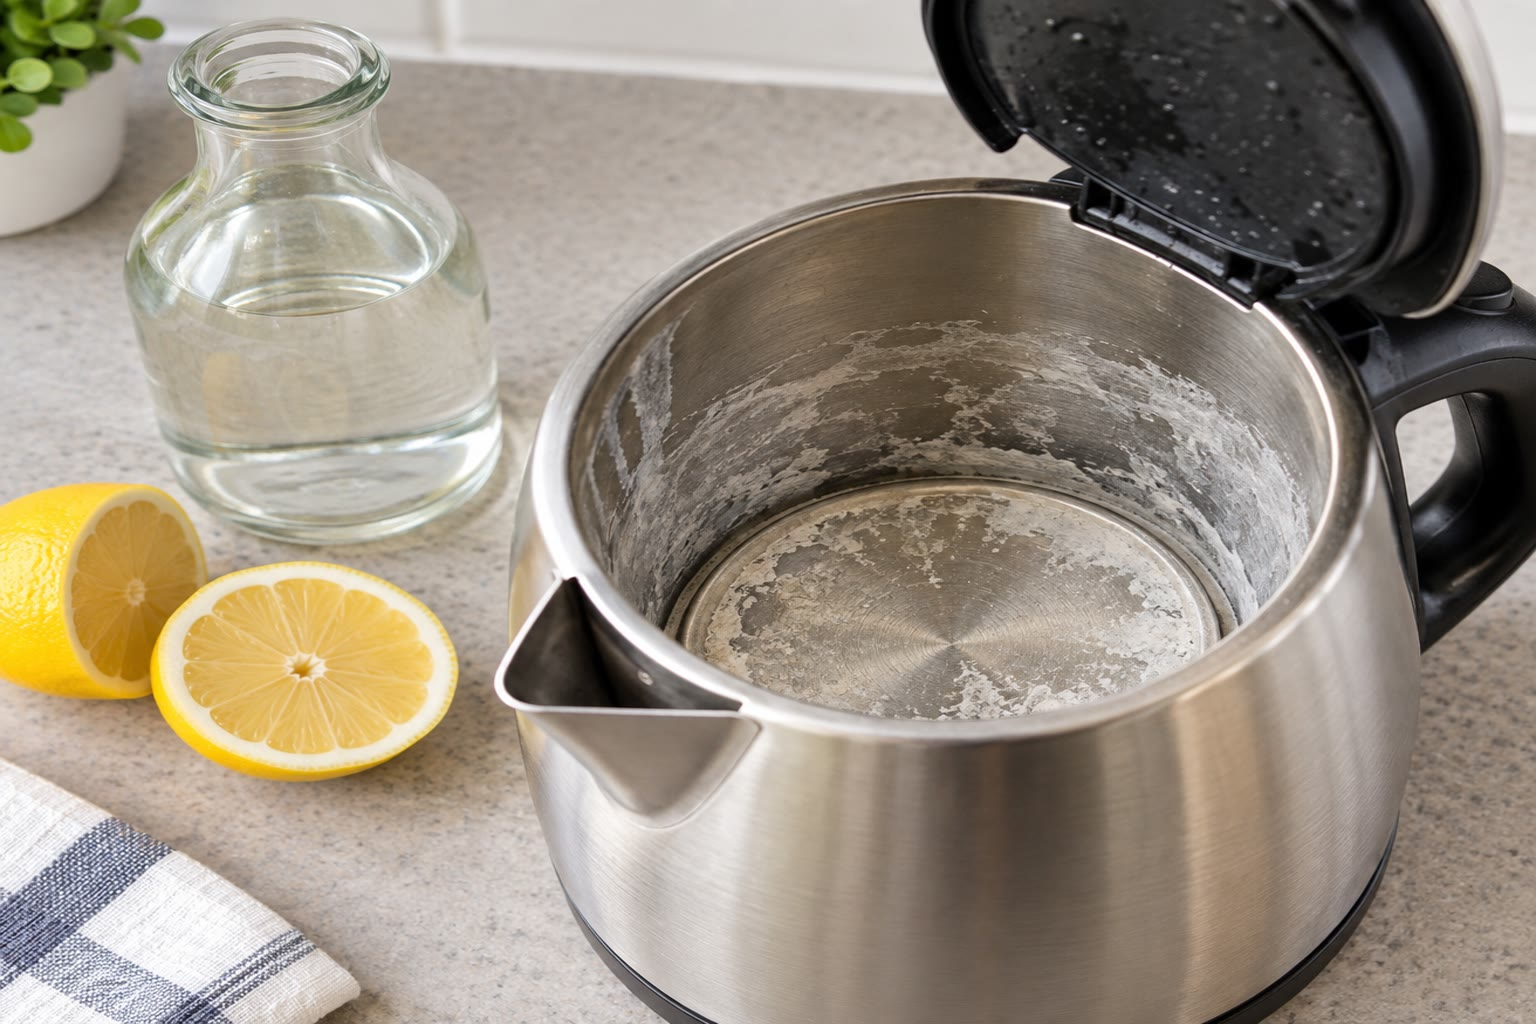
\includegraphics[width=0.5\linewidth]{images/book2/ai/b1-10-descaling.jpg}

{\small Kerak kapur, kalsium karbonat, di dalam ketel. Asam-asam lemah
cuka dan air jeruk lemon bereaksi dengan ion karbonat dan melarutkannya.}
\end{omfigure}

\section{Pasangan Brønsted dan pH}

\begin{definition}[Asam dan basa Brønsted, pasangan]\label{def:b1:predominant-reaction:bronsted}
\emph{Asam Brønsted}\index{asam Brønsted} adalah spesies yang mampu
memberikan proton \ce{H+}; \emph{basa Brønsted}\index{basa Brønsted}
adalah spesies yang mampu menerimanya. Asam HA dan basa A yang
terbentuk darinya dengan melepaskan sebuah proton membentuk
\emph{pasangan asam--basa}\index{pasangan asam--basa} HA/A, yang
dihubungkan oleh setengah reaksi formal $\mathrm{HA} \rightleftharpoons
\mathrm{A} + \ce{H+}$. Di dalam air proton tidak pernah bebas: proton itu
dibawa oleh sebuah molekul air sebagai \ce{H3O+}.
\end{definition}

\begin{definition}[Amfolit]\label{def:b1:predominant-reaction:ampholyte}
\emph{Amfolit}\index{amfolit} (spesies amfoter) adalah basa sebuah
pasangan dan sekaligus asam pasangan lain: air (\ce{H3O+}/\ce{H2O} dan
\ce{H2O}/\ce{OH-}), ion hidrogenkarbonat (\ce{CO2,H2O}/\ce{HCO3-} dan
\ce{HCO3-}/\ce{CO3^{2-}}), ion dihidrogenfosfat.
\end{definition}

\begin{definition}[Autoprotolisis, hasil kali ion, pH]\label{def:b1:predominant-reaction:autoprotolysis}
Air mengalami \emph{autoprotolisis}\index{autoprotolisis},
\ce{2H2O <=> H3O+ + OH-}, dengan tetapan $K_e = [\ce{H3O+}][\ce{OH-}]$,
yaitu \emph{hasil kali ion air}\index{hasil kali ion air}; pada
\qty{25}{\celsius}, $K_e = 10^{-14.00}$, sehingga $\mathrm{p}K_e = 14.00$.
pH sebuah larutan adalah $\mathrm{pH} = -\log a(\ce{H3O+}) \approx -\log[\ce{H3O+}]$.
Sebuah larutan netral jika $[\ce{H3O+}] = [\ce{OH-}]$, yaitu pada
$\mathrm{pH} = \mathrm{p}K_e/2 = 7.00$ pada \qty{25}{\celsius}.
% ledger: dfg:H2O_l, dfg:OH-_ao (pKe computed in figdata/bachelor-1/aqueous-constants.py)
\end{definition}

\section{Kekuatan: \texorpdfstring{$K_a$}{Ka}, \texorpdfstring{p$K_a$}{pKa}, dan efek perataan}

\begin{definition}[Tetapan keasaman]\label{def:b1:predominant-reaction:acidity-constant}
\emph{Tetapan keasaman}\index{tetapan keasaman} sebuah pasangan HA/A
adalah tetapan reaksi asam itu dengan air,
\[
  \mathrm{HA} + \ce{H2O} \rightleftharpoons \mathrm{A} + \ce{H3O+}, \qquad
  K_a = \frac{[\mathrm{A}][\ce{H3O+}]}{[\mathrm{HA}]}, \qquad
  \mathrm{p}K_a = -\log K_a .
\]
Makin besar $K_a$ (makin kecil $\mathrm{p}K_a$), makin kuat asamnya dan
makin lemah basa konjugasinya.
\end{definition}

\begin{definition}[Asam dan basa kuat dan lemah]\label{def:b1:predominant-reaction:strong-acid}
Sebuah asam disebut \emph{kuat}\index{asam kuat} di dalam air jika
reaksinya dengan air tuntas: tidak ada molekul HA yang tersisa (asam
klorida, asam nitrat, asam perklorat, keasaman pertama asam sulfat); jika
tidak, asam itu \emph{lemah}\index{asam lemah}. Sebuah basa disebut
\emph{kuat}\index{basa kuat} jika reaksinya dengan air tuntas dan
menghasilkan \ce{OH-} (hidroksida, ion oksida, alkoksida), dan
\emph{lemah}\index{basa lemah} jika tidak.
\end{definition}

\begin{definition}[Efek perataan]\label{def:b1:predominant-reaction:levelling}
Di dalam air, setiap asam yang lebih kuat daripada \ce{H3O+} bereaksi
tuntas menghasilkan \ce{H3O+}, dan setiap basa yang lebih kuat daripada
\ce{OH-} bereaksi tuntas menghasilkan \ce{OH-}: kekuatannya tidak dapat
dibedakan. Inilah \emph{efek perataan}\index{efek perataan} oleh pelarut.
Asam dan \omterm{def:b1:predominant-reaction:strong-acid}{basa lemah} di dalam air mempunyai $0 < \mathrm{p}K_a < 14$, dan
pasangan-pasangan air sendiri ($\mathrm{p}K_a(\ce{H3O+}/\ce{H2O}) = 0$ dan
$\mathrm{p}K_a(\ce{H2O}/\ce{OH-}) = 14$) membatasi skala itu.
\end{definition}

\begin{center}
\small
\begin{tabular}{lll@{\hspace{2.5em}}lll}
\hline
pasangan & p$K_a$ & & pasangan & p$K_a$ & \\
\hline
\ce{HSO4-}/\ce{SO4^{2-}} & 1.99 & & \ce{CO2,H2O}/\ce{HCO3-} & 6.37 & \\
\ce{H3PO4}/\ce{H2PO4-} & 2.15 & & \ce{H2PO4-}/\ce{HPO4^{2-}} & 7.21 & \\
\ce{HF}/\ce{F-} & 3.16 & & \ce{HClO}/\ce{ClO-} & 7.55 & \\
\ce{HCOOH}/\ce{HCOO-} & 3.74 & & \ce{NH4+}/\ce{NH3} & 9.25 & \\
\ce{CH3COOH}/\ce{CH3COO-} & 4.76 & & \ce{C6H5OH}/\ce{C6H5O-} & 9.99 & \\
\ce{C6H5NH3+}/\ce{C6H5NH2} & 4.60 & & \ce{HCO3-}/\ce{CO3^{2-}} & 10.33 & \\
\ce{C6H5COOH}/\ce{C6H5COO-} & 4.21 & & \ce{CH3NH3+}/\ce{CH3NH2} & 10.66 & \\
\hline
\end{tabular}
\end{center}
% ledger: pka:methanoic, pka:ethanoic, pka:anilinium, pka:benzoic,
% pka:phenol, pka:methylammonium (IUPAC dataset); dfg:HSO4-_ao,
% dfg:SO42-_ao, dfg:H3PO4_ao, dfg:H2PO4-_ao, dfg:HPO42-_ao, dfg:HF_ao,
% dfg:F-_ao, dfg:CO2_ao, dfg:HCO3-_ao, dfg:CO32-_ao, dfg:HClO_ao,
% dfg:ClO-_ao, dfg:NH4+_ao, dfg:NH3_ao (pKa computed from NBS-82)

\section{Diagram predominansi dan diagram distribusi}

\begin{definition}[Diagram predominansi dan diagram distribusi]\label{def:b1:predominant-reaction:predominance}
Untuk pasangan HA/A, $\mathrm{pH} = \mathrm{p}K_a + \log([\mathrm{A}]/[\mathrm{HA}])$:
asamnya predominan ($[\mathrm{HA}] > [\mathrm{A}]$) untuk
$\mathrm{pH} < \mathrm{p}K_a$, basanya untuk $\mathrm{pH} > \mathrm{p}K_a$.
\emph{Diagram predominansi}\index{diagram predominansi} adalah sumbu pH
yang dibagi pada setiap $\mathrm{p}K_a$ menjadi daerah-daerah tempat
setiap bentuk predominan.
\emph{Diagram distribusi}\index{diagram distribusi} memberikan bagian setiap bentuk, $[\text{bentuk}]/C$, sebagai
fungsi pH.
\end{definition}

\begin{proposition}[Hubungan Henderson dan fraksi-fraksi]\label{prop:b1:predominant-reaction:henderson}
Untuk pasangan HA/A dengan konsentrasi total $C = [\mathrm{HA}] + [\mathrm{A}]$,
\[
  \mathrm{pH} = \mathrm{p}K_a + \log\frac{[\mathrm{A}]}{[\mathrm{HA}]}, \qquad
  \frac{[\mathrm{HA}]}{C} = \frac{1}{1 + 10^{\mathrm{pH} - \mathrm{p}K_a}}, \qquad
  \frac{[\mathrm{A}]}{C} = \frac{1}{1 + 10^{\mathrm{p}K_a - \mathrm{pH}}} .
\]
Pada jarak satu satuan pH dari $\mathrm{p}K_a$, bentuk minornya di bawah
10\,\% dari total; pada jarak dua satuan, di bawah 1\,\%.
\end{proposition}

\begin{proof}
Ambillah logaritma $K_a = [\mathrm{A}][\ce{H3O+}]/[\mathrm{HA}]$. Maka
$[\mathrm{A}]/[\mathrm{HA}] = 10^{\mathrm{pH}-\mathrm{p}K_a}$, dan membagi
$[\mathrm{HA}]$ dengan $[\mathrm{HA}] + [\mathrm{A}]$ menghasilkan
fraksi-fraksinya. Pada
$\mathrm{pH} = \mathrm{p}K_a + 1$, $[\mathrm{HA}]/C = 1/11 < 10\,\%$; pada
$+2$, $1/101$.
\end{proof}

\begin{omfigure}
\begin{tikzpicture}
\begin{axis}[name=e,
  width=0.48\linewidth, height=5.2cm, xmin=0, xmax=14, ymin=0, ymax=1.05,
  axis x line=bottom, axis y line=left, xlabel={pH}, ylabel={fraksi},
  xtick={0,2,4,6,8,10,12,14},
  tick label style={font=\small}, label style={font=\small}]
\addplot[omDef, thick] table[x=pH, y=HA] {figdata/out/bachelor-1-distribution-diagrams-ethanoic.dat};
\addplot[omThm, thick] table[x=pH, y=A] {figdata/out/bachelor-1-distribution-diagrams-ethanoic.dat};
\draw[dotted] (axis cs:4.76,0) -- (axis cs:4.76,0.5);
\node[omDef, font=\footnotesize, anchor=west] at (axis cs:0.3,0.3) {\ce{CH3COOH}};
\node[omThm, font=\footnotesize, anchor=east] at (axis cs:13.7,0.3) {\ce{CH3COO-}};
\node[font=\small, anchor=north west] at (axis cs:4.8,0.48) {4.76};
\end{axis}
\begin{axis}[at={(e.east)}, anchor=west, xshift=1.1cm,
  width=0.48\linewidth, height=5.2cm, xmin=0, xmax=14, ymin=0, ymax=1.05,
  axis x line=bottom, axis y line=left, xlabel={pH}, ylabel={fraksi},
  xtick={0,2,4,6,8,10,12,14},
  legend style={font=\scriptsize, draw=none, at={(0.5,1.04)}, anchor=south, legend columns=4},
  tick label style={font=\small}, label style={font=\small}]
\addplot[omDef, thick] table[x=pH, y=H3A] {figdata/out/bachelor-1-distribution-diagrams-phosphoric.dat};
\addplot[omMeth, thick] table[x=pH, y=H2A] {figdata/out/bachelor-1-distribution-diagrams-phosphoric.dat};
\addplot[omProp, thick] table[x=pH, y=HA] {figdata/out/bachelor-1-distribution-diagrams-phosphoric.dat};
\addplot[omThm, thick] table[x=pH, y=A] {figdata/out/bachelor-1-distribution-diagrams-phosphoric.dat};
\legend{\ce{H3PO4}, \ce{H2PO4-}, \ce{HPO4^{2-}}, \ce{PO4^{3-}}}

\end{axis}
\end{tikzpicture}

\begin{tikzpicture}[font=\small, >={Stealth}]
  \draw[->, thick] (0,0) -- (14.2*0.85,0) node[right] {pH};
  \foreach \x/\l in {2.15/2.15, 7.21/7.21, 12.34/12.34}
    \draw (\x*0.85,0.15) -- (\x*0.85,-0.15) node[below] {\l};
  \node[above] at (1.07*0.85,0.1) {\ce{H3PO4}};
  \node[above] at (4.68*0.85,0.1) {\ce{H2PO4-}};
  \node[above] at (9.78*0.85,0.1) {\ce{HPO4^{2-}}};
  \node[above] at (13.3*0.85,0.1) {\ce{PO4^{3-}}};
\end{tikzpicture}

{\small \omterm{def:b1:predominant-reaction:predominance}{Diagram distribusi} asam etanoat (kiri) dan asam fosfat (kanan),
serta \omterm{def:b1:predominant-reaction:predominance}{diagram predominansi} asam fosfat. Setiap perpotongan dua kurva yang
bertetangga terletak pada sebuah $\mathrm{p}K_a$; \omterm{def:b1:predominant-reaction:ampholyte}{amfolit} \ce{H2PO4-} dan
\ce{HPO4^{2-}} hampir menjadi satu-satunya bentuk di tengah daerahnya.}
\end{omfigure}

\section{Metode reaksi predominan}

\begin{proposition}[Tetapan reaksi asam--basa]\label{prop:b1:predominant-reaction:k-of-reaction}
Reaksi asam $\mathrm{HA}_1$ sebuah pasangan dengan basa $\mathrm{A}_2$
pasangan lain,
$\mathrm{HA}_1 + \mathrm{A}_2 \rightleftharpoons \mathrm{A}_1 + \mathrm{HA}_2$,
mempunyai tetapan
\[
  K = \frac{K_{a1}}{K_{a2}} = 10^{\,\mathrm{p}K_{a2} - \mathrm{p}K_{a1}} .
\]
Reaksi itu menguntungkan ($K > 1$) jika asamnya lebih kuat daripada asam
yang terbentuk ($\mathrm{p}K_{a1} < \mathrm{p}K_{a2}$), dan \omterm{def:b1:extent-q-and-k:quantitative}{kuantitatif}
(dalam arti \cref{met:b1:extent-q-and-k:quantitative}) jika selisih
$\mathrm{p}K_a$-nya melebihi sekitar 4.
\end{proposition}

\begin{proof}
Reaksi itu adalah jumlah $\mathrm{HA}_1 + \ce{H2O} \rightleftharpoons
\mathrm{A}_1 + \ce{H3O+}$ ($K_{a1}$) dan kebalikan $\mathrm{HA}_2 +
\ce{H2O} \rightleftharpoons \mathrm{A}_2 + \ce{H3O+}$ ($1/K_{a2}$);
\cref{prop:b1:extent-q-and-k:combine-k} menghasilkan $K = K_{a1}/K_{a2}$.
\end{proof}

\begin{definition}[Reaksi predominan, larutan ekuivalen]\label{def:b1:predominant-reaction:predominant-reaction}
Dalam larutan yang mengandung beberapa asam dan basa, \emph{reaksi
predominan}\index{reaksi predominan} adalah reaksi dengan tetapan
terbesar antara asam terkuat dan basa terkuat yang ada. Jika reaksi itu
\omterm{def:b1:extent-q-and-k:quantitative}{kuantitatif}, reaksi itu diperlakukan sebagai reaksi tuntas, dan larutan
itu diganti dengan \emph{larutan ekuivalen}\index{larutan ekuivalen}:
larutan yang diperoleh setelah reaksi ini selesai, yang pH-nya sama
dengan pH larutan sebenarnya.
\end{definition}

\begin{method}[Metode reaksi predominan]\label{met:b1:predominant-reaction:method}
Untuk menentukan pH dan komposisi sebuah larutan:
\begin{enumerate}
  \item daftarkan spesies-spesies yang dimasukkan (dan air), lalu
        tempatkan pasangan-pasangannya pada skala $\mathrm{p}K_a$, asam di
        satu sisi, basa di sisi lain;
  \item tentukan asam terkuat dan basa terkuat yang ada;
  \item jika tetapan reaksi keduanya besar ($K > 10^4$, atau
        $\Delta\mathrm{p}K_a > 4$), perlakukan reaksi itu sebagai reaksi
        tuntas dan tuliskan \omterm{def:b1:predominant-reaction:predominant-reaction}{larutan ekuivalennya}; kembali ke langkah 2;
  \item jika \omterm{def:b1:predominant-reaction:predominant-reaction}{reaksi predominan} mempunyai tetapan yang kecil, reaksi itu
        menentukan pH: tuliskan tabel kemajuannya dan selesaikan $Q = K$,
        biasanya dengan hipotesis bahwa \omterm{def:b1:extent-q-and-k:extent}{kemajuan reaksinya} kecil;
  \item periksalah hipotesis-hipotesisnya: spesies-spesies minor memang
        minor, dan reaksi-reaksi lain (termasuk \omterm{def:b1:predominant-reaction:autoprotolysis}{autoprotolisis} air) dapat
        diabaikan.
\end{enumerate}
\end{method}

\begin{omfigure}
\begin{tikzpicture}[font=\small, >={Stealth}]
  \draw[->, thick] (0,-0.3) -- (0,7.6) node[above] {p$K_a$};
  \foreach \y/\a/\b in {0/\ce{H3O+}/\ce{H2O}, 1.58/\ce{HF}/\ce{F-}, 2.38/\ce{CH3COOH}/\ce{CH3COO-},
      3.62/\ce{H2PO4-}/\ce{HPO4^{2-}}, 4.62/\ce{NH4+}/\ce{NH3}, 7/\ce{H2O}/\ce{OH-}} {
    \draw (-0.12,\y) -- (0.12,\y);
    \node[anchor=east] at (-0.2,\y) {\a};
    \node[anchor=west] at (0.2,\y) {\b};
  }
  \foreach \y/\l in {0/0, 1.58/3.16, 2.38/4.76, 3.62/7.21, 4.62/9.25, 7/14} \node[black!60, anchor=west] at (3.0,\y) {\l};
  \draw[->, omThm, thick] (-1.6,2.55) -- (1.2,4.45);
  \node[omThm, anchor=west, align=left] at (4.2,3.5) {asam bereaksi dengan basa\\mana pun di atasnya: $K > 1$};
  \node[anchor=south] at (-1.4,7.35) {asam};
  \node[anchor=south] at (1.2,7.35) {basa};
\end{tikzpicture}

{\small Sebuah skala $\mathrm{p}K_a$ (digambar dengan p$K_a$ membesar ke
atas; nilai-nilainya di sebelah kanan). Sebuah asam bereaksi secara
menguntungkan dengan basa mana pun yang terletak di atasnya pada skala:
di sini asam etanoat dengan amonia, $K = 10^{9.25 - 4.76} = 10^{4.49}$.}
\end{omfigure}

\begin{proposition}[pH larutan-larutan sederhana]\label{prop:b1:predominant-reaction:ph-formulas}
Pada konsentrasi $C$ (dalam \unit{mol/L}), dengan $\mathrm{p}C = -\log C$:
\begin{itemize}
  \item \omterm{def:b1:predominant-reaction:strong-acid}{asam kuat}: $\mathrm{pH} = \mathrm{p}C$, berlaku untuk
        $\mathrm{pH} < 6.5$;
  \item \omterm{def:b1:predominant-reaction:strong-acid}{asam lemah} yang sedikit terdisosiasi: $\mathrm{pH} = \frac12(\mathrm{p}K_a
        + \mathrm{p}C)$, berlaku jika $\mathrm{pH} < \mathrm{p}K_a - 1$;
  \item \omterm{def:b1:predominant-reaction:strong-acid}{basa lemah} yang sedikit terprotonasi: $\mathrm{pH} = \frac12(\mathrm{p}K_e +
        \mathrm{p}K_a - \mathrm{p}C)$, berlaku jika $\mathrm{pH} > \mathrm{p}K_a +
        1$;
  \item \omterm{def:b1:predominant-reaction:ampholyte}{amfolit} dengan $\mathrm{p}K_{a2} - \mathrm{p}K_{a1} > 4$:
        $\mathrm{pH} = \frac12(\mathrm{p}K_{a1} + \mathrm{p}K_{a2})$,
        berapa pun $C$ (asalkan tidak terlalu encer).
\end{itemize}
\end{proposition}

\begin{proof}
\omterm{def:b1:predominant-reaction:strong-acid}{Asam kuat}: \ce{HA + H2O -> A- + H3O+} tuntas, $[\ce{H3O+}] = C$, karena
sumbangan air sendiri ($10^{-7}$) dapat diabaikan jika $C > 10^{-6.5}$.
\omterm{def:b1:predominant-reaction:strong-acid}{Asam lemah}: \omterm{def:b1:predominant-reaction:predominant-reaction}{reaksi predominannya} adalah $\mathrm{HA} + \ce{H2O}
\rightleftharpoons \mathrm{A} + \ce{H3O+}$ dengan kemajuan $x = [\ce{H3O+}]
= [\mathrm{A}]$; jika $x \ll C$, $K_a = x^2/C$, $\mathrm{pH} = \frac12(\mathrm{p}K_a
+ \mathrm{p}C)$; hipotesis $[\mathrm{A}] < [\mathrm{HA}]/10$ setara dengan
$\mathrm{pH} < \mathrm{p}K_a - 1$. \omterm{def:b1:predominant-reaction:strong-acid}{Basa lemah}: sama, dengan $\mathrm{A} +
\ce{H2O} \rightleftharpoons \mathrm{HA} + \ce{OH-}$, yang tetapannya $K_e/K_a$.
\omterm{def:b1:predominant-reaction:ampholyte}{Amfolit} HA$^-$: \omterm{def:b1:predominant-reaction:predominant-reaction}{reaksi predominannya} adalah $2\,\mathrm{HA}^- \rightleftharpoons
\mathrm{H_2A} + \mathrm{A}^{2-}$, sehingga $[\mathrm{H_2A}] = [\mathrm{A}^{2-}]$;
mengalikan $K_{a1} = [\mathrm{HA}^-]h/[\mathrm{H_2A}]$ dengan $K_{a2} =
[\mathrm{A}^{2-}]h/[\mathrm{HA}^-]$ menghasilkan $h^2 = K_{a1}K_{a2}$.
\end{proof}

\begin{omfigure}
\begin{tikzpicture}
\begin{axis}[
  width=0.66\linewidth, height=5.6cm, xmin=0, xmax=8, ymin=0, ymax=8,
  axis x line=bottom, axis y line=left,
  xlabel={$\mathrm{p}C = -\log C$}, ylabel={pH},
  xtick={0,1,2,3,4,5,6,7,8}, ytick={0,1,2,3,4,5,6,7,8},
  tick label style={font=\small}, label style={font=\small},
  legend style={font=\small, draw=none, at={(0.02,0.98)}, anchor=north west}]
\addplot[omDef, very thick] table[x=pC, y=pH] {figdata/out/bachelor-1-weak-acid-ph.dat};
\addplot[omProp, dashed] table[x=pC, y=weak] {figdata/out/bachelor-1-weak-acid-ph.dat};
\addplot[black!50, dotted, thick] table[x=pC, y=strong] {figdata/out/bachelor-1-weak-acid-ph.dat};
\draw[black!30] (axis cs:0,7) -- (axis cs:8,7);
\legend{eksak, $\frac12(\mathrm{p}K_a + \mathrm{p}C)$, $\mathrm{pH} = \mathrm{p}C$}
\end{axis}
\end{tikzpicture}

{\small pH larutan asam etanoat terhadap $\mathrm{p}C$, yang dihitung
secara eksak dari neraca muatan. Jika pekat, asamnya sedikit
terdisosiasi dan mengikuti $\frac12(\mathrm{p}K_a + \mathrm{p}C)$; jika
diencerkan di bawah sekitar $10^{-6}$ mol/L, asam itu terdisosiasi
sempurna dan berperilaku sebagai \omterm{def:b1:predominant-reaction:strong-acid}{asam kuat}; jika sangat encer, pH-nya
menuju 7.}
\end{omfigure}

\begin{example}[Asam etanoat dan amonia]\label{ex:b1:predominant-reaction:mixture}
Campurkan \qty{0.10}{mol} asam etanoat dan \qty{0.10}{mol} amonia dalam
\qty{1.0}{L}. Asam terkuat adalah \ce{CH3COOH}, basa terkuat
\ce{NH3}: \ce{CH3COOH + NH3 <=> CH3COO- + NH4+}, $K = 10^{9.25 - 4.76} =
10^{4.49}$, \omterm{def:b1:extent-q-and-k:quantitative}{kuantitatif}. \omterm{def:b1:predominant-reaction:predominant-reaction}{Larutan ekuivalennya} mengandung
\qty{0.10}{mol/L} \ce{CH3COO-} dan \ce{NH4+}. \omterm{def:b1:predominant-reaction:predominant-reaction}{Reaksi predominannya}, yaitu
\ce{NH4+ + CH3COO- <=> NH3 + CH3COOH}, mempunyai tetapan yang kecil,
$10^{-4.49}$, dan menjaga $[\ce{NH3}] = [\ce{CH3COOH}]$, sehingga, seperti
untuk \omterm{def:b1:predominant-reaction:ampholyte}{amfolit}, $\mathrm{pH} = \frac12(4.76 + 9.25) = 7.01$.
\end{example}

\section{Asam poliprotik dan larutan penyangga}

\begin{definition}[Asam poliprotik]\label{def:b1:predominant-reaction:polyprotic}
\emph{Asam poliprotik}\index{asam poliprotik} dapat memberikan beberapa
proton secara berturut-turut, setiap tahap dengan tetapannya sendiri:
asam fosfat \ce{H3PO4} ($\mathrm{p}K_a$ = 2.15, 7.21, 12.34), asam
karbonat (\ce{CO2,H2O}; 6.37, 10.33), asam sulfat (keasaman pertama kuat,
kedua 1.99). Nilai-nilai $\mathrm{p}K_a$ berturut-turut membesar:
melepaskan proton dari spesies yang sudah bermuatan negatif lebih mahal.
\end{definition}

\begin{example}[Asam fosfat \texorpdfstring{\qty{0.10}{mol/L}}{0.10 mol/L}]\label{ex:b1:predominant-reaction:h3po4}
\omterm{def:b1:predominant-reaction:predominant-reaction}{Reaksi predominannya} adalah keasaman pertama. Dengan $x = [\ce{H3O+}]$,
$x^2/(0.10 - x) = 10^{-2.15}$; di sini $x$ tidak kecil dibandingkan
dengan $C$, sehingga persamaan kuadrat $x^2 + K_{a1}x - K_{a1}C = 0$
diselesaikan: $x =
\qty{0.0233}{mol/L}$, $\mathrm{pH} = 1.63$. Keasaman kedua
($\mathrm{p}K_{a2} = 7.21$) tidak menyumbang apa pun pada pH ini.
\end{example}

\begin{definition}[Larutan penyangga]\label{def:b1:predominant-reaction:buffer}
\emph{Larutan penyangga}\index{larutan penyangga} adalah larutan yang
pH-nya hanya sedikit berubah jika sedikit asam atau basa ditambahkan,
atau jika larutan itu diencerkan. Penyangga yang biasa adalah campuran
\omterm{def:b1:predominant-reaction:strong-acid}{asam lemah} dan basa konjugasinya dalam jumlah yang sebanding; pH-nya
mendekati $\mathrm{p}K_a$ pasangan itu.
\end{definition}

\begin{proposition}[Mengapa penyangga bertahan]\label{prop:b1:predominant-reaction:buffer}
Untuk penyangga yang terdiri atas $n_a$ mol asam dan $n_b$ mol basa,
$\mathrm{pH} =
\mathrm{p}K_a + \log(n_b/n_a)$ tidak bergantung pada volume.
Penambahan $\delta$ mol \omterm{def:b1:predominant-reaction:strong-acid}{asam kuat} mengubahnya sebesar
\[
  \Delta\mathrm{pH} = \log\frac{n_b - \delta}{n_a + \delta} - \log\frac{n_b}{n_a}
  \approx -\frac{\delta}{\ln 10}\left(\frac{1}{n_a} + \frac{1}{n_b}\right),
\]
yang paling kecil untuk $n_a = n_b$ pada jumlah total tertentu.
\end{proposition}

\begin{proof}
\omterm{def:b1:predominant-reaction:strong-acid}{Asam kuat} bereaksi tuntas dengan basa: $n_b \to n_b - \delta$,
$n_a \to n_a + \delta$. Turunan $f(\delta) = \log(n_b - \delta) -
\log(n_a + \delta)$ di 0 adalah $-\frac{1}{\ln10}\big(\frac{1}{n_b} +
\frac{1}{n_a}\big)$; untuk $n_a + n_b$ tetap, $\frac1{n_a} + \frac1{n_b}$
paling kecil jika $n_a = n_b$.
\end{proof}

\begin{definition}[Derajat disosiasi]\label{def:b1:predominant-reaction:dissociation}
\emph{Derajat disosiasi}\index{derajat disosiasi} sebuah \omterm{def:b1:predominant-reaction:strong-acid}{asam lemah} HA
pada konsentrasi analitis $C$ adalah $\alpha = [\mathrm{A}]/C$, yaitu
bagian asam yang terdisosiasi oleh air; derajat disosiasi memenuhi
hukum pengenceran Ostwald $\alpha^2C/(1 - \alpha) = K_a$, dan menuju 1
ketika $C \to 0$.
\end{definition}

\begin{inthelab}[Membuat larutan penyangga]
Di laboratorium, penyangga dibuat dengan menimbang asam dan garamnya
(misalnya natrium dihidrogenfosfat dan dinatrium hidrogenfosfat), atau
dengan menambahkan volume larutan natrium hidroksida yang terukur ke
dalam asamnya sambil membaca pH meter yang telah dikalibrasi sebelumnya
dengan dua \omterm{def:b1:predominant-reaction:buffer}{larutan penyangga} standar; larutan itu lalu diencerkan sampai
tanda batas di dalam labu ukur.
\end{inthelab}

\section{Latihan}

\begin{exercise}[$\star$]\label{exo:b1:predominant-reaction:1}
Tuliskan basa konjugasi \ce{H2SO4}, \ce{HCO3-}, \ce{NH4+}, dan \ce{H2O},
serta asam konjugasi \ce{NH3}, \ce{HPO4^{2-}}, \ce{OH-}, dan \ce{H2O}.
Manakah di antara spesies-spesies ini yang merupakan \omterm{def:b1:predominant-reaction:ampholyte}{amfolit}?
\end{exercise}

\begin{exercise}[$\star$]\label{exo:b1:predominant-reaction:2}
Dengan tabel $\mathrm{p}K_a$, urutkan asam fluorida, asam etanoat, ion
amonium, dan asam hipoklorit menurut kekuatannya, lalu tentukan $K_a$
masing-masing.
\end{exercise}

\begin{exercise}[$\star$]\label{exo:b1:predominant-reaction:3}
Hitunglah pH larutan asam klorida \qty{0.010}{mol/L}, dan larutan
natrium hidroksida \qty{0.010}{mol/L}, pada \qty{25}{\celsius}.
\end{exercise}

\begin{exercise}[$\star$]\label{exo:b1:predominant-reaction:4}
Gambarlah \omterm{def:b1:predominant-reaction:predominance}{diagram predominansi} pasangan \ce{CH3COOH}/\ce{CH3COO-}.
Bentuk manakah yang predominan dalam minuman ringan ber-pH 3, dan dalam
darah ber-pH 7.4? Berapa bagian asam yang berada dalam bentuk asam pada
pH 3.76?
\end{exercise}

\begin{exercise}[$\star\star$]\label{exo:b1:predominant-reaction:5}
Hitunglah pH larutan amonia \qty{0.10}{mol/L} dan periksalah hipotesis
yang dibuat.
\end{exercise}

\begin{exercise}[$\star\star$]\label{exo:b1:predominant-reaction:6}
Hitunglah pH larutan asam etanoat \qty{0.010}{mol/L} dan \omterm{def:b1:predominant-reaction:dissociation}{derajat
disosiasinya}; periksalah hipotesisnya.
\end{exercise}

\begin{exercise}[$\star\star$]\label{exo:b1:predominant-reaction:7}
Tuliskan \omterm{def:b1:predominant-reaction:predominant-reaction}{reaksi predominan}, tetapannya, dan pH larutan yang diperoleh
dengan mencampurkan, dalam \qty{1.0}{L}, \qty{0.10}{mol} asam fluorida
dan \qty{0.050}{mol} natrium hidroksida.
\end{exercise}

\begin{exercise}[$\star\star$]\label{exo:b1:predominant-reaction:8}
Sebuah penyangga mengandung \qty{0.050}{mol} asam etanoat dan
\qty{0.050}{mol} natrium etanoat dalam \qty{1.0}{L}. Hitunglah pH-nya,
lalu pH sesudah penambahan \qty{0.010}{mol} asam klorida. Bandingkan
dengan penambahan yang sama ke dalam \qty{1.0}{L} air murni.
\end{exercise}

\begin{exercise}[$\star\star$]\label{exo:b1:predominant-reaction:9}
Asam klorida dan asam nitrat sama kuat di dalam air, tetapi tidak di
dalam asam etanoat murni sebagai pelarut. Jelaskan, lalu sebutkan asam
terkuat yang dapat ada di dalam air.
\end{exercise}

\begin{exercise}[$\star\star\star$]\label{exo:b1:predominant-reaction:10}
Hitunglah pH larutan natrium karbonat \qty{0.10}{mol/L}, dan periksalah
bahwa kebasaan kedua dapat diabaikan.
\end{exercise}

\begin{exercise}[$\star\star\star$]\label{exo:b1:predominant-reaction:11}
Buktikan hukum pengenceran Ostwald dan hitunglah \omterm{def:b1:predominant-reaction:dissociation}{derajat disosiasi} asam
etanoat pada $C = \qty{1.0e-3}{mol/L}$. Mengapa pendekatan
$\alpha \ll 1$ gagal di sini?
\end{exercise}

\begin{exercise}[$\star\star\star$]\label{exo:b1:predominant-reaction:12}
Sebuah larutan mengandung \qty{0.010}{mol/L} asam klorida dan
\qty{0.10}{mol/L} asam etanoat. Tentukan pH-nya dan konsentrasi ion
etanoat; jelaskan mengapa \omterm{def:b1:predominant-reaction:strong-acid}{asam lemah} itu hampir tidak terdisosiasi.
\end{exercise}

\section{Soal: Penyangga Fosfat untuk Laboratorium Kultur Sel}

\begin{problem}[{Soal akhir pekan --- tiga keasaman asam fosfat, pH
ketiga garam natriumnya, larutan ekuivalen, dan volume natrium hidroksida
yang menghasilkan penyangga ber-pH 7.20}]
\label{pb:b1:predominant-reaction:1}
Sel-sel yang dikultur di laboratorium memerlukan medium dengan pH
mendekati 7.2. Data pada \qty{25}{\celsius}: $\mathrm{p}K_a$ asam fosfat
2.15, 7.21, dan 12.34; $\mathrm{p}K_e = 14.00$.

\medskip
\noindent\textbf{Bagian I --- Asam fosfat.}
\begin{enumerate}
  \item Tuliskan ketiga pasangan dan setengah reaksinya.
  \item Gambarlah \omterm{def:b1:predominant-reaction:predominance}{diagram predominansi} asam fosfat.
  \item Spesies manakah yang predominan pada pH 1, 5, 9, dan 13?
  \item Spesies manakah yang merupakan \omterm{def:b1:predominant-reaction:ampholyte}{amfolit}?
  \item Mengapa setiap $\mathrm{p}K_a$ lebih besar daripada yang
        sebelumnya?
\end{enumerate}

\medskip
\noindent\textbf{Bagian II --- Tiga larutan \qty{0.100}{mol/L}.}
\begin{enumerate}[resume]
  \item Untuk asam fosfat, tuliskan \omterm{def:b1:predominant-reaction:predominant-reaction}{reaksi predominannya} dan tunjukkan
        bahwa \omterm{def:b1:extent-q-and-k:extent}{kemajuan reaksinya} tidak dapat diabaikan dibandingkan
        dengan $C$.
  \item Hitunglah pH larutan asam fosfat itu.
  \item Untuk natrium dihidrogenfosfat \ce{NaH2PO4}, tuliskan \omterm{def:b1:predominant-reaction:predominant-reaction}{reaksi
        predominan} dan tetapannya.
  \item Hitunglah pH larutan ini.
  \item Hitunglah pH larutan dinatrium hidrogenfosfat \ce{Na2HPO4}.
  \item Manakah di antara ketiga larutan itu yang paling dekat dengan pH
        yang diinginkan?
\end{enumerate}

\medskip
\noindent\textbf{Bagian III --- Menambahkan natrium hidroksida.}
Sebuah larutan mengandung \qty{0.100}{mol} \ce{H3PO4}; ke dalamnya
ditambahkan $n$ mol natrium hidroksida, dengan volume total
\qty{1.00}{L}.
\begin{enumerate}[resume]
  \item Tuliskan reaksi \qty{0.100}{mol} hidroksida yang pertama beserta
        tetapannya. Apakah reaksi itu \omterm{def:b1:extent-q-and-k:quantitative}{kuantitatif}?
  \item Paparkan \omterm{def:b1:predominant-reaction:predominant-reaction}{larutan ekuivalen} untuk $n = \qty{0.100}{mol}$ dan
        tentukan pH-nya.
  \item Pertanyaan yang sama untuk $n = \qty{0.150}{mol}$.
  \item Pertanyaan yang sama untuk $n = \qty{0.200}{mol}$.
  \item Sketsalah pH sebagai fungsi $n$ dari 0 sampai \qty{0.300}{mol}.
  \item Mengapa larutan pada pertanyaan 14 merupakan penyangga yang baik?
\end{enumerate}

\medskip
\noindent\textbf{Bagian IV --- Membuat \qty{1.00}{L} penyangga ber-pH 7.20.}
Tersedia natrium hidroksida \qty{1.00}{mol/L}.
\begin{enumerate}[resume]
  \item Rasio $[\ce{HPO4^{2-}}]/[\ce{H2PO4-}]$ berapakah yang menghasilkan
        pH 7.20?
  \item Nyatakan jumlah \ce{H2PO4-} dan \ce{HPO4^{2-}} dalam jumlah $x$
        hidroksida yang ditambahkan melebihi \qty{0.100}{mol} pertama.
  \item Hitunglah $x$.
  \item Seberapa besar pH berubah jika \qty{1.0e-3}{mol} asam klorida
        ditambahkan ke dalam penyangga ini? ke dalam \qty{1.00}{L} air
        murni?
  \item Apakah pH akan berubah jika penyangga itu diencerkan sepuluh
        kali? Jelaskan.
  \item Hitunglah volume larutan natrium hidroksida yang harus
        ditambahkan ke dalam \qty{0.100}{mol} asam fosfat untuk
        memperoleh \qty{1.00}{L} penyangga ber-pH 7.20.
\end{enumerate}
\end{problem}
